\documentclass[11pt,a4paper]{paper} 
\usepackage[pdftex]{graphicx}
\usepackage{subfig}
\usepackage{moreverb}
\usepackage[table]{xcolor}
%\usepackage{subfig}
%\usepackage{subfigure}
\author{David Voong}
\title{Offline alignment of the RICH system:  \\ tracking of the HPD image centre. 2011 Update}
\begin{document} 
\maketitle
%\tableofcontents

%Needs a lot of work. Remember this is aimed at a non-expert so you need to explain everything. Think that a new PhD student is going to take over your work and needs to understand in detail what has been done so far. 
%
%You need to be far more quantitative in your discussions of figures etc.

%%%%%%%%%%%%%%%%%%%%%%%%%%%%%%%%%%%%%%%%%%%%%%%%%%%%%%%%%%%%%%%%%%%%%%%%
%                                                                                   		INTRODUCTION													        %
%%%%%%%%%%%%%%%%%%%%%%%%%%%%%%%%%%%%%%%%%%%%%%%%%%%%%%%%%%%%%%%%%%%%%%%%
\section{Introduction}
%1. What is an HPD
%2. What is its purpose
%3. Layout and dimensions
%4. Operation
%5. Performance
The Hybrid photon detectors (HPD) are used to detect Cherenkov photons emitted by particles traversing the RICH system. The hit positions of the emitted photons form a ring on the HPD plane, the radius of which is related to the Cherenkov angle associated to the particle. The Cherenkov angle of a particle acts as a signature of its particle type. This enables discrimination between electrons, pions, kaons and protons which is needed to identify the decay processes of particles produced in the LHCb detector. 

The HPDs are arrange in two grids, for RICH 1 [RICH 2] the grids are positioned above [left] and below [right] the beamline and are are arranged into rows of $14$ [$16$] by $7$ [$9$] columns (Fig \ref{fig: RICH 1: upper grid}). The HPDs are approximately cylindrical in shape, with a length of $160\,\mathrm{mm}$ and radius of $43.7\,\mathrm{mm}$ \footnote{There are small differences in the dimensions of the HPDs in RICH1 and RICH2. The values given here are for the HPDs in RICH 1, details for the HPDs in RICH 2 can be found in the RICH Technical design report.} (See Fig \ref{fig: HPD schematic} and Fig \ref{fig:HPD_photo}). A spherically-shaped cap quartz window is attached to one end of the HPD, on its inner surface is a deposition of an S20 (multi alkali) photo-cathode which emits photo-electrons when stimulated by photons. The emitted photo-electrons traverse the vacuum chamber of the HPD where they are accelerated an electric potential difference of $20\,\mathrm{kV}$ onto a square silicon chip array of $32\,\times\,32$ pixels \footnote{When the HPD is run is its ALICE configuration the pixel dimensions are $32\,\times\,256$ pixels} with a length and width of $16\,\mathrm{mm}$.

\begin{figure}
	\begin{center}
		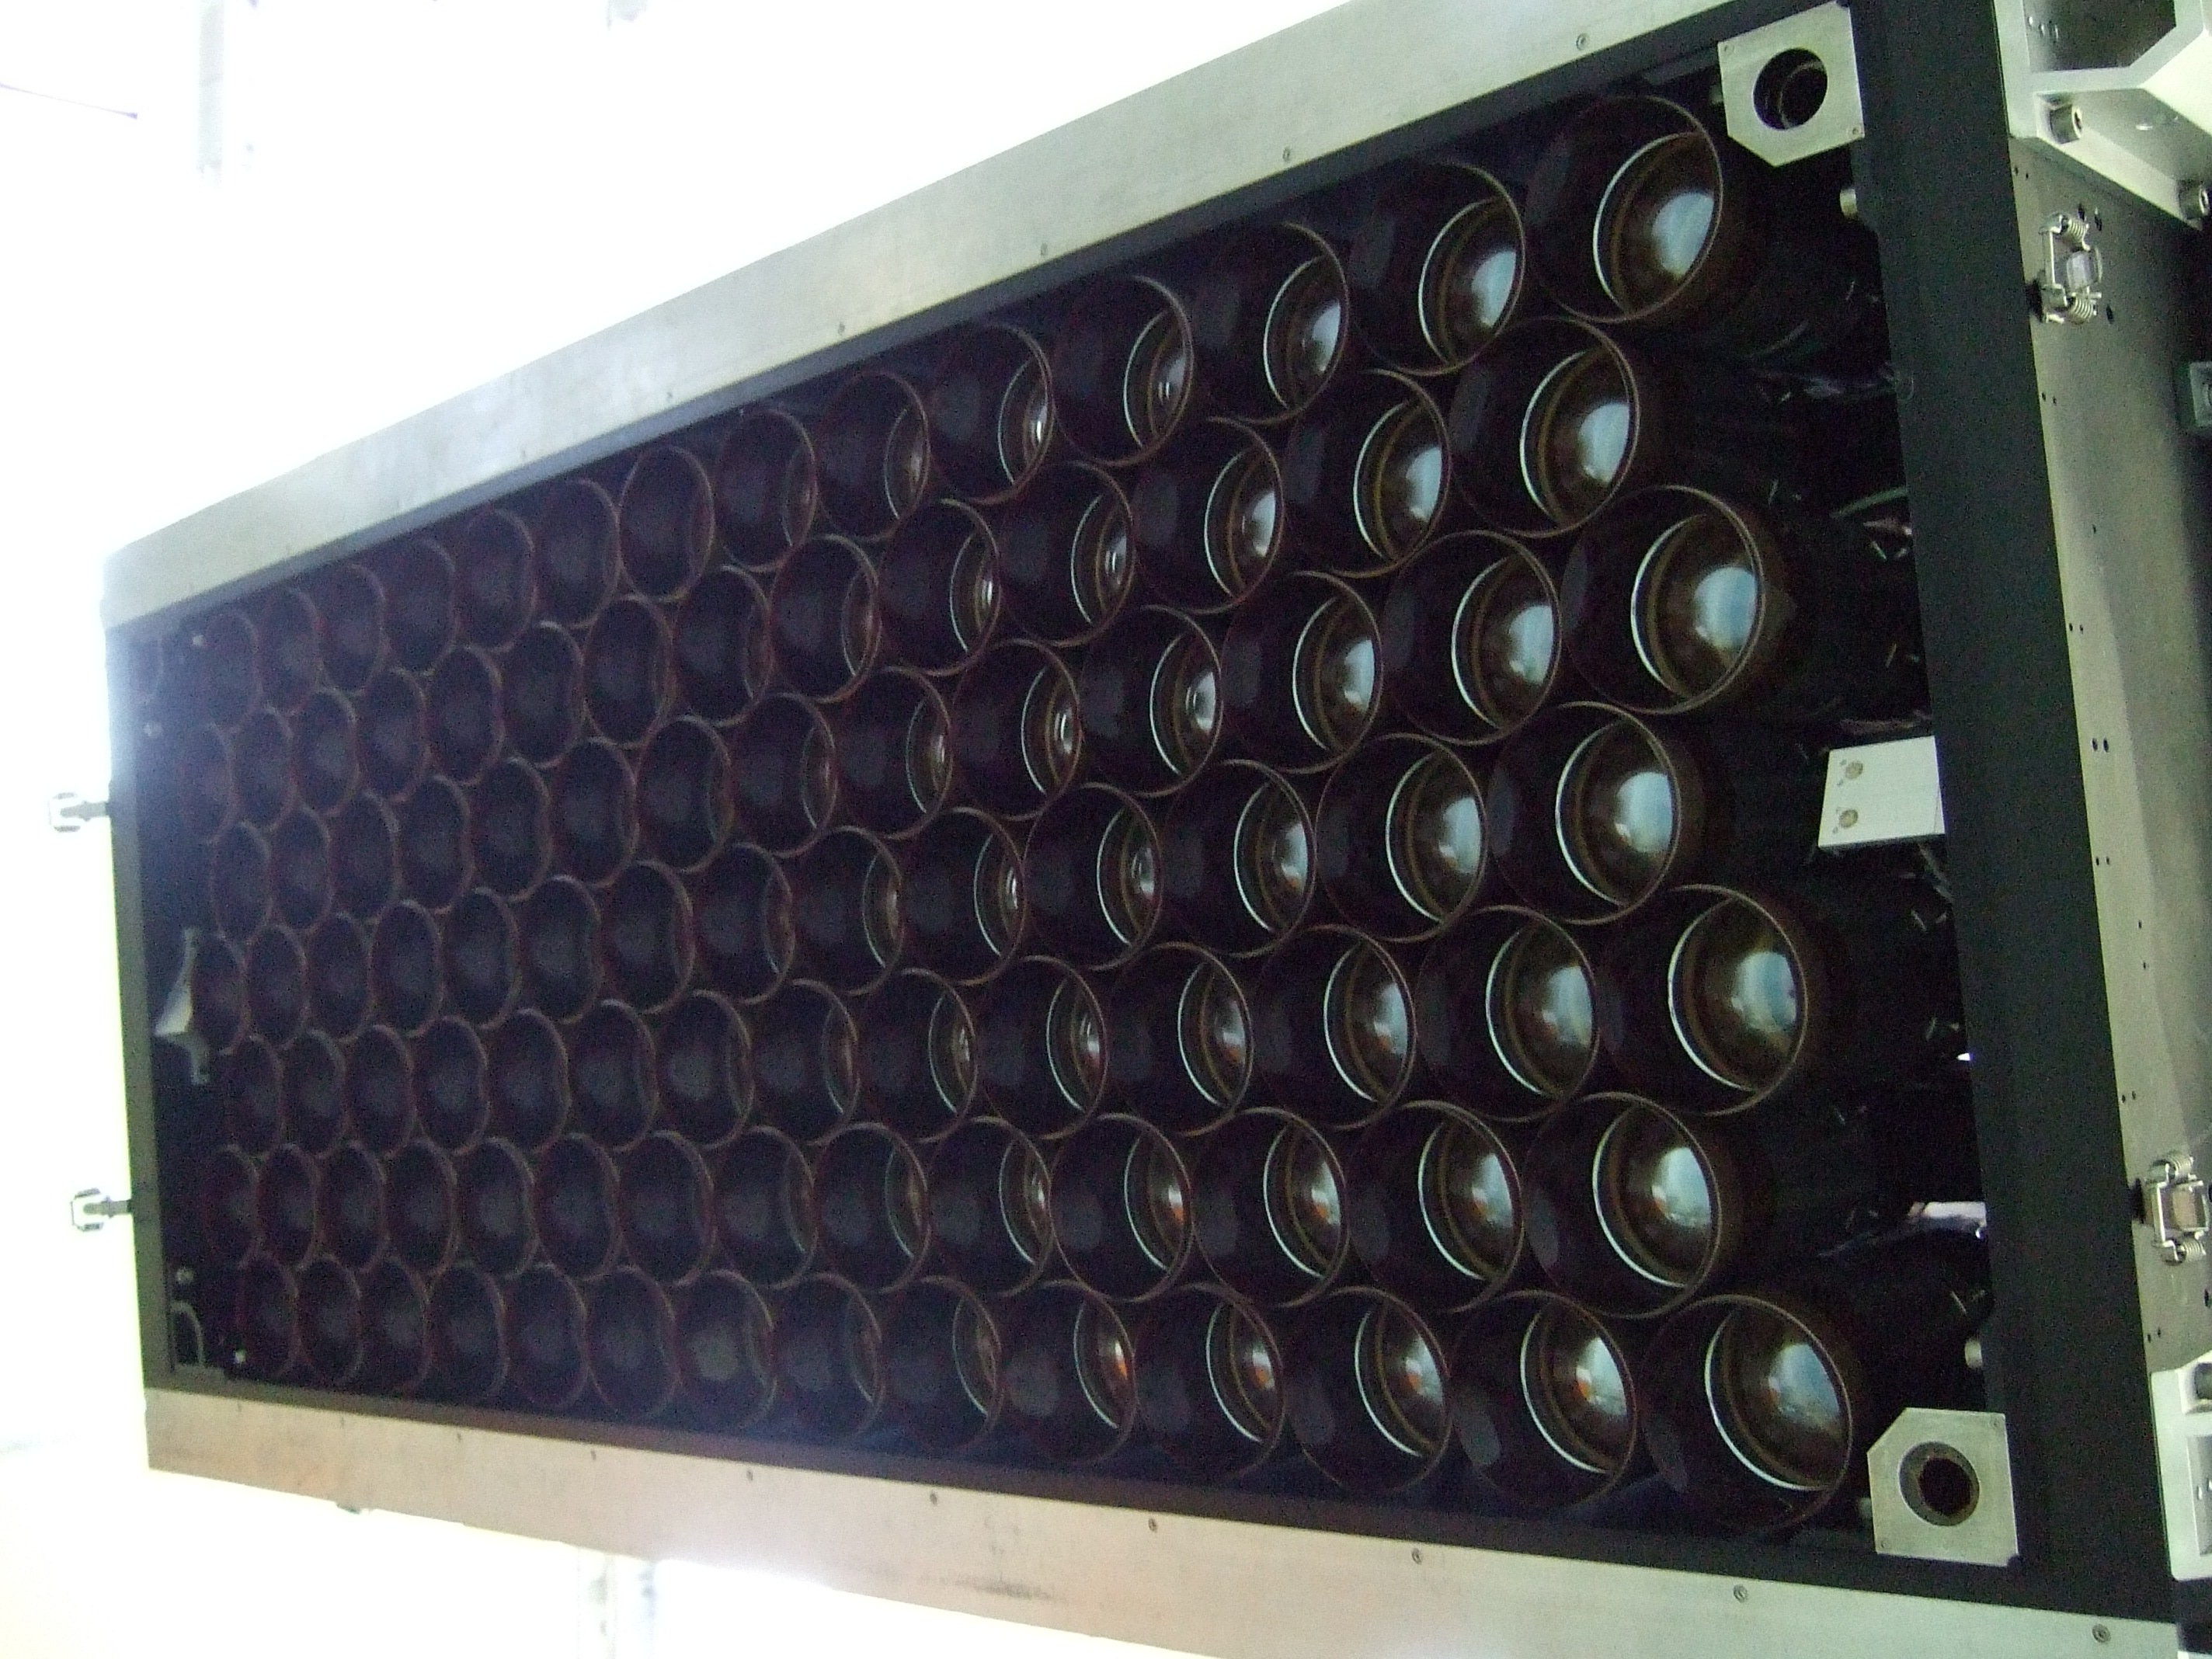
\includegraphics[width=0.5\columnwidth]{../images/RICH1_Upper_box_134.jpg}
		\caption{Upper HPD grid in RICH 1}
		\label{fig: RICH 1: upper grid}
	\end{center}
\end{figure}

\begin{figure}
	\begin{minipage}[b]{0.45\linewidth}
		\centering
			\includegraphics[height=4cm, width=6cm]{$HOME/Dropbox/LHCb/detector/RICH/images/HPD_schematic2.png}
			\caption{HPD schematic}
			\label{fig: HPD schematic}
	\end{minipage}
	\hspace{0.5cm}
	\begin{minipage}[b]{0.45\linewidth}
		\centering
		\includegraphics[height=4cm]{$HOME/Dropbox/LHCb/detector/RICH/images/HPD_photo.jpg}
		\caption{photo of a HPD}
		\label{fig:HPD_photo}
	\end{minipage}
\end{figure}

The total accumulation of pixel signals over the course of a run can be visualised on a two dimensional plot called a hit map (or image summary fig \ref{example_HPD_image_summaries}). Due to the circular shape of the quartz window the hit map is circular in shape. An image centre is determined by fitting a circle to the boundary of the hit map and taking the central position. The accuracy in the position of the image centre is an important property of the HPD since any translation of the image centre effects the accuracy in the position of the photon, Cherenkov angle and particle identification. 

\begin{figure}
	\begin{center}
		\includegraphics[width=13cm]{$HOME/Dropbox/LHCb/detector/RICH/images/HPD_image_summaries.png}
		\caption{Example HPD hit maps for HPDs 001, 002 and 092 for run 80168. The z-axis corresponds to the number of hits registered by a pixel, the x and y axes correspond to the pixel position on the silicon chip}
		% comment: Either change the naming convention of the HPDs to match U half / D half notation and include image of layout of include image of numbered naming convention
		\label{example_HPD_image_summaries}
	\end{center}
\end{figure}

Observations of the image centre show that its position does not necessarily line up with the centre of the silicon chip, this effect is accounted for by an alignment process which reflects the displacement of the image centre from the silicon chip centre in the detector description of the LHCb detector. In addition, during the course of operation, shifts in the position of the image centre for individual HPDs have been consistently observed. These shifts can be as much as $2\,\mathrm{mm}$ (Fig \ref{fig: shift_distance}) between consecutive runs. This phenomenon was further confirmed during and investigation carried out in laboratory tests performed at the end of 2009 using HPDs removed from the LHCb detector for which shifts has been most noticeably observed. The low levels of mechanical stress, scale of the shifts (Fig \ref{fig: 2010 displacement}) and rigidity of the HPD fixings suggest the image shifts are not due to physical movement of the HPD components, but are instead the result of disturbances to the electric fields due to build up of charge on HPD components over the duration of operation. Additionally shifts were shown to be present across both magnetic field configurations and when the magnet was off suggesting this effect was not an artefact of the magnet.

In addition to the alignment of the HPD image centres the performance of the RICH detector is also dependent on the alignment of its other components. In particular the alignment of the mirrors which reflect the Cherenkov radiation onto the HPD plane and the Magnetic distortion monitoring system (MDCS) which corrects distortion effects to the HPDs due to the magnetic field from the LHCb magnet. These alignment procedures are intimately entangled such that changes in any of the alignment procedures will effect the other. Since improvements in the individual alignment systems are constantly ongoing in parallel it can be difficult to disentangle how the effect of changes in the individual alignment systems effects the RICH system as a whole. 

The work presented here builds on alignment techniques performed previously for the data collected in 2010 developed. The main changes were to introduce a run by run time dependence on the alignment method. For the data taking period of 2010 the HPD image centres were calculated by averaging over the whole year. Improvements were also made to the general stability and accuracy of the fit. At the time of writing the current alignment software produces improvements $\sim7\%$ in RICH1 and RICH2 (section \ref{chap: application of correction factors}) compared to the 2010 alignment techniques.

\begin{figure}
%	\centering
	\begin{center}
	\caption{Image centre x,y displacement and shifts for 2010 tagged consecutive runs ranging from 68179 - 80168}
	\label{fig: 2010 displacement}
		\subfloat[x-displacement]
		{
			\label{fig: x_displacement}
			\includegraphics[width=.7\columnwidth]{/afs/cern.ch/user/d/dvoong/analysis/rich/HPDs/image_fitting/displacement_between_conseq_runs/scripts/x_displacement.png}
		}
		\\
		\subfloat[y-displacement]
		{
			\label{fig: y_displacement}	
			\includegraphics[width=.7\columnwidth]{/afs/cern.ch/user/d/dvoong/analysis/rich/HPDs/image_fitting/displacement_between_conseq_runs/scripts/y_displacement.png}
		}
		\\
		\subfloat[shift distance]
		{
			\label{fig: shift_distance}
			\includegraphics[width=.7\columnwidth]{/afs/cern.ch/user/d/dvoong/analysis/rich/HPDs/image_fitting/displacement_between_conseq_runs/scripts/shift_distance.png}
		}
	\end{center}
\end{figure}

%Photons incident to the HPD plane in the RICH system pass first through the quartz window of an individual HPD (fig \ref{fig: HPD schematic}). The quartz window is a spherically-shaped cap with a radius of $40\,\mathrm{mm}$ providing a photosensitive area with a radius of $36\,\mathrm{mm}$. Photons are focused by the curvature of the quartz window towards the centre of the HPD cavity. An S20(multi-alkali) photo-cathode deposition on the inner surface results in the emission of photo-electrons into the vacuum chamber of the HPD.  These are then accelerated by an electric field across a potential difference of $20\,\mathrm{kV}$ onto a square silicon chip array of $32 \,\times\, 32$ pixels with a  width and length of $16\,\mathrm{mm}$.

%\begin{figure}
%\begin{center}
%	\subfloat[HPD schematic]
%	{
%%		\includegraphics[height=4cm, width=6cm]{$HOME/Dropbox/LHCb/detector/RICH/images/HPD_schematic2.png}
%		\includegraphics[height=4cm, width=6cm]{$HOME/Dropbox/LHCb/detector/RICH/images/HPD_schematic2.png}
%		\label{fig: HPD schematic}
%	}
%	\subfloat[photo of a HPD]
%	{
%		\includegraphics[height=4cm]{$HOME/Dropbox/LHCb/detector/RICH/images/HPD_photo.jpg}
%		
%	}
%\caption{}
%\label{HPD_schematic}
%
%\end{center}
%\end{figure}

%Figure \ref{fig: shift_distance} shows the distribution of the image centre displacement for all consecutive runs of all HPDs. Figure \ref{fig: x_displacement} and figure \ref{fig: y_displacement} show the image centre displacements in x and y respectively.
%Due to the support structure and scale of the shifts (Fig \ref{fig: 2010 displacement}) in the HPDs it is unlikely that these shifts are due to the physical shift of the components of the HPDs. They also are not due to distortion effects from the magnet in the LHCb detector; laboratory tests of HPDs taken from sub-detector at the end of 2009 showed that the shifts were present when no magnetic field was present.
%
% also, shifts are seen  but rather an effective shift due disturbances in the electric field. 
%
%Shifts in the image centre have been observed consistently both during running of the LHCb detector and under laboratory conditions during testing. The order of these shifts can be as much as $2\,\mathrm{mm}$ (Fig \ref{fig:shift_distance}) between consecutive runs resulting in significant effects on the resolution of the Cherenkov angle. Due to the support structure, fixings present and scale of the shifts (Fig \ref{fig: 2010 displacement}) in the HPDs it is unlikely that these shifts are due to the physical shift of the components of the HPDs but rather an effective shift due disturbances in the electric field. Current theories attribute this to electrostatic fields arising from the gradual build up of charge on components of the HPD. Regardless of cause the motion of image centres are a very real effect with significant effects on the performance of the RICH system.
%Though the shifts are not thought to be due to the physical motion of components, instead only an effective shift,  the procedure treats them as such. The correction procedure tracks the motion of the shifts and updates the LHCb conditions database accordingly on a run by run basis.

%Image centre shifts are not to be confused with effects related to magnetic distortions originating from the external magnetic field produced by the LHCb magnet (which are corrected for by the MDCS [Magnetic Distortion Calibration System]) since image centre shifts have also been observed in conditions where the magnetic field is off (there is however some degree of non-trivial entanglement between the two phenomena in the case where the magnet is on)
%It is also unlikely that the shifts are due to physical movements of the HPD components due to the scale of the effect (see figure \ref{fig: 2010 displacement}) .
%
%The most plausible cause for this phenomenon is believed to be due to electrostatic disturbances coming from electromagnet fields produce by the gradual build of charge on the components of the HPD.
%
%I guess it's not the chip that is moving but the image i.e. distortion of the electrostatic forces
%
%To correct for this effect the shift is considered as an effective movement in the position of the silicon chip relative to the other central axis of the HPD. THe image centre positions are calculated and recorded in the LHCb Conditions database path below for each run.
%
%\begin{verbatim}
%/Conditions/Rich1/Alignment/SiSensorsP0.xml
%\end{verbatim}
%with entries of the form,
%
%\begin{verbatim}
%<!-- HPD hardwareID H637010  Copy# 39 
%2011-RootFiles-RunAligned-Sobel-AveragePol0-HPDAlign-26082011-->
%<condition classID="6" name="SiSensor39_Align">
%   <paramVector name="dPosXYZ" type="double">
%      0.3510891980990485 0.1097093608556504 0
%   </paramVector>
%   <paramVector name="dRotXYZ" type="double">
%      0 0 0
%   </paramVector>
%   <paramVector name="pivotXYZ" type="double">
%      0 0 0
%   </paramVector>
%</condition>
%\end{verbatim}

%Need to discuss things in a quantitative way. Discuss the t the size of shifts that would trigger an update of the conditions and how regularly such shifts are observed
%I don't think the conditions are updated depending on the the size of the shifts but more as a function of time. Operation time is correlated to the number of hits, which correlated to the accuracy of circle fit. But shorter periods are correlated to a better resolution in the tracking of the image centre. Weigh up benefits and detriments/disadvantages. 

%%%%%%%%%%%%%%%%%%%%%%%%%%%%%%%%%%%%%%%%%%%%%%%%%%%%%%%%%%%%%%%%%%%%%%%%
%                                                                                   FIRST OBSERVATION OF IMAGE SHIFTS								 		        %
%%%%%%%%%%%%%%%%%%%%%%%%%%%%%%%%%%%%%%%%%%%%%%%%%%%%%%%%%%%%%%%%%%%%%%%%
\section{First observation of image shifts}
The shifting of images was first noticed in the middle of 2009 most noticeably in a HPD located around the outer corner (HPD: A7 13) of the the A-side HPD plane (Fig \ref{fig: RICH2_HPD_plane_layout}). The RICH2 HPD intervention in October 2009 was used as an opportunity to extract the HPD to investigate image shifts in a laboratory environment. 

The set up for the laboratory tests were chosen so that the conditions were as similar as possible to the conditions in the LHCb detector. Tests were performed over time periods varying from 48 to 450 hours using an LED light source. Figure \ref{fig: november lab test} shows the results from a 48 hour period test, Figure \ref{fig: thierry row} [\ref{fig: thierry col}] shows the variation in the row [column] position of the image centre and figure \ref{fig: thierry radius} shows the variation in the radius of the circle used to fit the HPD hit map. In January 2010 the tests were repeated over a 450 hour period to investigate whether the shifts exhibited oscillatory behaviour, results are shown in figure \ref{fig: january lab test}, no significant repeating behaviour was observed.

\begin{figure}
	\begin{center}
		\subfloat[image centre row position, note: lab test were performed with HPD in Alice mode meaning a greater number of effective pixels on the chip (8 Alice pixels to 1 LHCb pixel (0.5mm))]
		{
			\includegraphics[width=0.7\columnwidth]{$HOME/Dropbox/LHCb/detector/RICH/HPDs/alignment/thierry_stuff/november_lab_tests/pngs/row_position.png}
			\label{fig: thierry row}
		} \, \\
%		\hspace{2mm}
		\subfloat[image centre column position]
		{
			\includegraphics[width=0.7\columnwidth]{$HOME/Dropbox/LHCb/detector/RICH/HPDs/alignment/thierry_stuff/november_lab_tests/pngs/column_position.png}
			\label{fig: thierry col}
		} \, \\
		\subfloat[image radius]
		{
			\includegraphics[width=0.7\columnwidth]{$HOME/Dropbox/LHCb/detector/RICH/HPDs/alignment/thierry_stuff/november_lab_tests/pngs/radius.png}
			\label{fig: thierry radius}
		}
		\caption{HPD A7 13 image shift lab test results over a period of four days}
		\label{fig: november lab test}
	\end{center}
\end{figure}

\begin{figure}
	\includegraphics[width=\columnwidth]{../images/january_lab_test.png}
	\caption{HPD image centre shift laboratory tests in January 2010. HPDs image shifts were monitored over a 450 hour period}
	\label{fig: january lab test}
\end{figure}

\newpage

%%%%%%%%%%%%%%%%%%%%%%%%%%%%%%%%%%%%%%%%%%%%%%%%%%%%%%%%%%%%%%%%%%%%%%%%
%                                                                                   		IMAGE FITTING TECHNIQUE											        %
%%%%%%%%%%%%%%%%%%%%%%%%%%%%%%%%%%%%%%%%%%%%%%%%%%%%%%%%%%%%%%%%%%%%%%%%
\section{Image fitting technique}
\label{section: Fitting Procedure}

Image fitting is applied to the accumulated hit maps in order to find the centre of the image. A boundary finding procedure is first employed to find the edges of the images, once the boundary is determined a $\chi^2$ minimisation is performed to fit a circle to the boundary. Various boundary finding methods were investigated, two of these are outline below, 1. Threshold boundary fitting and 2. Sobel boundary fitting.

%Shifts in the image centre translate to a shift in the effective position of the silicon chip sensor. From this it follows that if this shift is not corrected for then some error will be associated to projection of photons on the HPD hence their Cherenkov angles. This is corrected by modifying the LHCb detector database to include information on the HPD image centre positions (translated to the silicon chip position). Since the image centre positions vary with time it is necessary to to split the database up into slices such that each slice corresponds to a run period.

%The alignment procedure involves fitting the HPD hit map (fig \ref{example_HPD_image_summaries}), this involves first marking out a boundary to the image which is then fitted with a circle from which the centre is taken as the image centre. %, this is followed by a correction to the image centre to compensate for the displacement from its nominal position. This steps of this process are outlined below,

%\begin{enumerate}
%	\item Calculate an image boundary for the hit map
%	\item Fit a circle to the image boundary and take the centre of the circle as the centre of the hit map
%	\item Record image centre in the LHCb conditions database with a timestamp corresponding to the time of the run
%	\item Rerun the reconstruction software with the updated conditions database for the end of year reprocessing (Since the hit map is produced from data collected over the total duration of a run it is not possible to perform an online alignment at the time of data taking)
%\end{enumerate}

%A private database together with a full RICH reconstruction was carried out to test the effect of the alignment procedure on the Cherenkov angle resolution.

%%%%%%%%%%%%%%%%%%%%%%%%%%%%%%%%%%%%%%%%%%%%%%%%%%%%%%%%%%%%%%%%%%%%%%%%
%                                                                                   		BOUNDARY SELECTION PROCEDURE									        %
%%%%%%%%%%%%%%%%%%%%%%%%%%%%%%%%%%%%%%%%%%%%%%%%%%%%%%%%%%%%%%%%%%%%%%%%
\subsection {Boundary selection procedure}
The boundary selection method uses an iterative algorithm to scan over the hit map scanning from the pixels in the outer region towards the centre. A test is applied to each pixel with a set of criteria to meet, the outermost pixels which pass the test are then marked as part of the boundary of the image. The Sobel boundary fitting method incorporates and additional process is applied to the hit map prior to the boundary selection, this process emphasises regions in the image with large changes to the image intensity hence emphasising the image boundaries.


%The alignment software provides two different methods for fitting the image centre of a HPD hit map. These correspond to the two different methods for fitting the boundary (the circle fitting procedure for the two methods is the same). The two boundary fitting methods are outlined in the following sections.

%The boundary of the image can be calculated by two possible methods which are outlined in the following sections. In general the boundary selection method uses an iterative algorithm to scan over the hit map scanning from the pixels in the outer region towards the centre. A test is applied to each pixel with a set of criteria to meet, the outermost pixels which pass the test are marked as part of the boundary of the image. 

%, the criteria are as follows,
%The boundary of the image can be calculated by two possible methods, these are outlined in the following sections.
%The algorithm can be configured to scan the image in various orders, e.g. columns followed by rows and vice-versa.


%%%%%%%%%%%%%%%%%%%%%%%%%%%%%%%%%%%%%%%%%%%%%%%%%%%%%%%%%%%%%%%%%%%%%%%%
%                                                                                   		THRESHOLD BOUNDARY FITTING										        %
%%%%%%%%%%%%%%%%%%%%%%%%%%%%%%%%%%%%%%%%%%%%%%%%%%%%%%%%%%%%%%%%%%%%%%%%
\subsubsection{Threshold boundary fitting}

The threshold boundary method uses two criteria to determine the boundary pixels.

\begin{description}
	\item[Criteria 1] \hfill \\ The number of hits for a pixel must pass a user defined threshold parameter. The parameter is defined such that a value of 1 corresponds to the average number of hits per pixel for the HPD image. The optimal threshold value is calculated by comparing the Cherenkov angle resolution as a function of the threshold value.
	\item[Criteria 2] \hfill \\ At least one of its adjacent pixels must also pass requirement 1, this requirement reduces the contribution of pixels with unexpectedly high population (noisy pixels). This can occur when there is a fault with an individual pixel.
\end{description}

%The threshold boundary fitting method carries on from the 2010 alignment software approach, the simpler of the two methods, it involves an iterative algorithm which effectively scans over the pixel map on the silicon chip scanning from the outer regions of the chip to the centre. The first pixel to satisfy the following requirements marks the a boundary point on the HPD image summary,

%The threshold boundary method uses an iterative algorithm to scan over the hit map scanning from the pixels in the outer region towards the centre. A test is applied to each pixel with a set of criteria to meet, the outermost pixels which pass the test are marked as part of the boundary of the image, the criteria are as follows, 

%comment: Need some plots of boundary selection using threshold method
%In the 2010 software the boundary algorithm scanned {\bf only} the from top to bottom and from bottom to top of the HPD. The 2011 software additional scans horizontally and determines a boundary from the convolution of both directions. The differences can be seen in figure \ref{fig: comparison of 2010, 2011 boundary fitting}
%Needs more detail of what I'm looking at in the Figure.
%\begin{figure}[ht]
%	\begin{center}
%	\subfloat[2010]
%	{
%		\includegraphics[height = 4cm, width = 4cm]{/Users/admin/Pictures/scruffy_dog_small.jpg}
%		\label{fig:simple boundary fitting 2010}
%	}
%	\subfloat[2011]
%	{
%		\includegraphics[height = 4cm, width = 4cm]{/Users/admin/Pictures/scruffy_dog_small.jpg}
%		\label{fig:simple boundary fitting 2011}
%	}
%	\caption{Comparison of simple boundary fitting 2010 and 2011} 
%	\label{fig: simple boundary fitting comparison}
%	\end{center}
%\end{figure}

%\begin{figure}
%\begin{center}
%\includegraphics[width=13cm]{$HOME/Dropbox/LHCb/detector/RICH/images/boundary_fitting_comparison.pdf}
%\caption{Boundary fitting comparison: left) 2010, centre) HPD image summary with image cleaning and Sobel filter applied, right) HPD image summary with fitted circle of centre image overlaid}
%\label{fig: comparison of 2010, 2011 boundary fitting}
%\end{center}
%\end{figure}

% Put image of 2010 boundary fitting here too

%\begin{figure}
%\begin{center}
%\includegraphics[width=13cm]{$HOME/Dropbox/LHCb/detector/RICH/images/HPD_image_summaries_boundary.png}
%\caption{HPD image summaries from figure \ref{example_HPD_image_summaries} with boundaries fitted using the 2011 simple boundary fitting method}
%\label{fig: simple boundary fitting 2011}
%\end{center}
%\end{figure}

% figures showing the boundary fitting algorithm for 2010 and 2011


%%%%%%%%%%%%%%%%%%%%%%%%%%%%%%%%%%%%%%%%%%%%%%%%%%%%%%%%%%%%%%%%%%%%%%%%
%                                                                                   		SOBEL BOUNDARY FITTING										        	        %
%%%%%%%%%%%%%%%%%%%%%%%%%%%%%%%%%%%%%%%%%%%%%%%%%%%%%%%%%%%%%%%%%%%%%%%%
\subsubsection{Sobel boundary fitting}


Similarly to the threshold boundary method the Sobel method also uses a set of criteria to select a boundary, however, before this process a filter is applied to the HPD hit image which maps the intensity ($I$) of a pixel to its intensity gradient in relation to its adjacent pixels. An example of the Sobel filter being used in the field of image processing can be seen in figure \ref{fig: sobel example} and an example of the application of the Sobel filter to a HPD image is shown in figure \ref{fig: HPD image with Sobel filter applied}. The intensity gradient is calculated by calculating the horizontal and vertical intensity gradients for a pixel and combining them using Pythagoras theorem,

\begin{equation}
	\frac{\partial I}{\partial \vec{r}} \approx \sqrt{\left(\frac{\partial I}{\partial x}\right)^2 + \left(\frac{\partial I}{\partial y}\right)^2}
\end{equation}

For a pixel located on row $i$ and column $j$ the horizontal intensity gradient is given by, 

\begin{equation}
	\left(\frac{\partial I}{\partial x}\right)_{(i,j)} = (I_{(i+1,j-1)} - I_{(i+1, j+1)}) + 2(I_{(i,j-1)} - I_{(i, j+1)}) + (I_{(i-1,j-1)} - I_{(i-1, j+1)})
\end{equation}

where the first term is equal to the difference between the lower diagonal left and lower diagonal right pixels; the second term is the difference between the left and right pixels weighted by a factor of two; the third term is the difference between the upper diagonal left and upper diagonal right pixels. Similarly for the the vertical intensity gradient,

\begin{equation}
	\left(\frac{\partial I}{\partial y}\right)_{(i,j)} = (I_{(i-1,j+1)} - I_{(i+1, j+1)}) + 2(I_{(i-1,j)} - I_{(i+1, j)}) + (I_{(i-1,j-1)} - I_{(i+1, j-1)})
\end{equation}

where the first term is difference between the lower diagonal left and upper diagonal left pixels; the second term is difference between the lower and upper pixels weighted by a factor of two; the third term is difference between the lower diagonal right and upper diagonal right pixels.

A boundary finding algorithm is then applied to the filtered hit map, the boundary pixels are required to match the following criteria,

\begin{description}
	\item[Criteria 1] \hfill \\ The intensity gradient of a pixel must pass a user defined threshold parameter. The optimal threshold value is calculated by comparing the Cherenkov angle resolution as a function of the threshold value.
	\item[Criteria 2]\hfill \\ The pixel must be either a peak pixel (adjacent pixels on the same column or row must have a lower intensity gradient) or be adjacent to a peak pixel and have an intensity gradient greater than a user defined threshold value that is related to the intensity gradient of its corresponding peak pixel.
\end{description}

An example of the boundary finding algorithm can be seen in figure \ref{fig: comparison of 2010, 2011 boundary fitting}.

\begin{figure}[h]
	\begin{center}
		\includegraphics[width=13cm]{$HOME/Dropbox/LHCb/detector/RICH/images/sobel_example.png}
		\caption{An example of the Sobel filter in action}
		\label{fig: sobel example}
	\end{center}
\end{figure}

\begin{figure}[h]
	\begin{center}
		\includegraphics[width=13cm]{$HOME/Dropbox/LHCb/detector/RICH/images/Sobel_filtered_image.png}
		\caption{HPD image summary with Sobel filter applied}
		\label{fig: HPD image with Sobel filter applied}
	\end{center}
\end{figure}

%This can be visualised as 
%
%In the case of the horizontal intensity gradient this  taking the difference between intensities of adjacent pixels on the left and right columns and summing this with the difference between the intensities of the diagonally left and right pixels for the above and below rows. In addition the pixels on the central row contribute more to the intensity gradient and are given a weight of twice that for the diagonals. The weighting for the horizontal intensity gradient is visualised below, \\

%Qualitatively this is equivalent to, in the case of the horizontal intensity gradient, taking the difference between intensities of adjacent pixels on the left and right and summing this with the difference between the intensities of the diagonally left and right pixels for the above and below rows. In addition the pixels on the central row contribute more to the intensity gradient and are given a weight of twice that for the diagonals. The weighting for the horizontal intensity gradient is visualised below, \\

%\begin{center}
%$
%	\left( \begin{array}{ccc}
%	-1 & 0 & 1 \\
%	-2 & 0 & 2 \\
%	-1 & 0 & 1 \end{array} \right)
%$
%\end{center}
%
%Similarly in the case of the vertical intensity gradient, the intensity gradient is given by the difference between intensities of adjacent pixels on the top and bottom and summing this with the difference between the intensities of the diagonally top and bottom pixels for the left and right columns. Again the weighting is different for each column.
%
%\begin{center}
%$
%	\left( \begin{array}{ccc}
%	-1 & -2 & -1 \\
%	 0 &  0  &  0  \\
%	 1 &  2  &  1 \end{array} \right)
%$
%\end{center}

%Again what I'm I looking at Fig 2.3
%The Sobel method is the default method for boundary fitting, it has been shown to significant improve on the threshold boundary method. The Sobel method involves first applying the Sobel operator to the hit map. For a generic image the application of the Sobel operator produces a map of image intensity gradients (fig \ref{sobel example}). In the case of the HPD image this corresponds to the variation in the intensity of hits on the pixels on the silicon chip. The result of this can be seen in fig \ref{fig: HPD image with Sobel filter applied}. The peak regions in the image intensity gradient map correspond to the boundary region of the unprocessed image, the problem of finding the boundary of the unprocessed image is then simplified to finding the peak regions in image gradient map.

%%%

%\subsection{The Sobel operator}
%\label{sec: the Sobel operator}
%The Sobel operator is a discrete differentiation operator, computing an approximation of the gradient of the image intensity function.
%Defining A as the image source, $*$ is the convolution operator and $G_x$, $G_y$ as the respective gradients of the image we have,
%\begin{center}
% \[
% G_x =  
%\left( \begin{array}{ccc}
%-1 & 0 & 1 \\
%-2 & 0 & 2 \\
%-1 & 0 & 1 \end{array} \right) * A 
%\]
%\[ 
%G_y =  
%\left( \begin{array}{ccc}
%-1 & -2 & -1 \\
%0 & 0 & 0 \\
%1 & 2 & 1 \end{array} \right) * A 
%\]  \\
%\[
%G = \sqrt{G_x^2 + G_y^2} 
%\] \newline
%
%\end{center}
%
%In the case of the vertical operator the operation on a pixel at $(x_1, y_1)$  calculates the intensity difference between the above and below pixels weighted by two summed with the intensity difference of the above right and below right pixels and of the top left and bottom left pixel both weighted by a factor of 1. \newline
%
%\begin{table}[htdp]
%\begin{center}
%\begin{tabular}{|c|c|c|}
%\hline
%{\cellcolor[gray]{0.8}} & {\cellcolor[gray]{0.}} & {\cellcolor[gray]{0.8}} \\ 
%\hline
% &  &  \\ 
%\hline
%{\cellcolor[gray]{0.8}} & {\cellcolor[gray]{0}} & {\cellcolor[gray]{0.8}} \\
%\hline
%\end{tabular}
%\caption{the vertical intensity gradient of the centre pixel is calculated by summing the difference between the respective pixels in the above and below rows. The black pixels are weighted by a factor of 2 and the grey are weighted by a factor of 1}
%\end{center}
%\end{table}%
%
%$dI(x_1, y_1)/dy \approx 2\times \{I(x_1, y_1+1) - I(x_1, y_1-1)\} + \{I(x_1+1, y_1+1) - I(x_1+1, y_1-1)\} + \{I(x_1-1, y_1+1) - I(x_1+1, y_1-1)\} $

%%%

%alternatively, relative to a non-edge pixel with image intensity $I$, \newline
%\begin{center}
%
%$\frac{\partial I(n,m)}{\partial x} \approx I(n+1, m+1) - I(n+1, m-1) + 2*(I(n, m+1)-I(n, m-1)) + I(n-1, m+1) - I(n-1, m-1)$ \newline
%
%$\frac{\partial I(n,m)}{\partial y} \approx I(n-1, m-1) - I(n+1, m-1) + 2*(I(n-1, m)-I(n+1, m)) + I(n-1, m+1) - I(n+1, m+1)$ \newline
%
%$\frac{\partial I(n,m)}{\partial r} \approx \sqrt{\frac{\partial I(n,m)}{\partial x}^2 + \frac{\partial I(n,m)}{\partial y}^2}$ \newline

%$\frac{\partial I}{\partial x} \approx I_{top\,right} - I_{top\,left} + 2*(I_{right} - I_{left}) + I_{bottom\,right} - I_{bottom\,left} $ \newline
%
%$\frac{\partial I}{\partial y} \approx I_{bottom,left} - I_{top\,left} + 2*(I_{bottom} - I_{top}) + I_{bottom\,right} - I_{top\,right}$ \newline
%
%\[
%\frac{\partial I}{\partial r} \approx \sqrt{\frac{\partial I}{\partial x}^2 + \frac{\partial I}{\partial y}^2}
%\]
%
%$r = \sqrt{x^2 + y^2}$

%\end{center}

%A lot more detail needed in this section outlining the method. As a non-expert I'm afraid I'm non the wiser of what's going on having read the section


 
 %%%%%
 
 \newpage
 
%%%%%%%%%%%%%%%%%%%%%%%%%%%%%%%%%%%%%%%%%%%%%%%%%%%%%%%%%%%%%%%%%%%%%%%%
%                                                                                   		CIRCLE FITTING										        	        		        %
%%%%%%%%%%%%%%%%%%%%%%%%%%%%%%%%%%%%%%%%%%%%%%%%%%%%%%%%%%%%%%%%%%%%%%%%
\subsection{Circle fitting}
The circle fitting procedure is carried out by minimising the chi squared function,
\begin{equation}
 \chi^2(x_0, y_0, r) = \sum \limits_{n=0}^{N}\left(\sqrt{(x_n-x_0)^2 + (y_n-y_0)^2} - r\right)^2 \cdot I_n
\end{equation}
where $x_0$ and $y_0$ correspond to the x and y coordinates of the centre of the circle, $r$ the radius and $(x_n, y_n, I_n)$ are the $x$, $y$ coordinates and intensity for the boundary pixel $n$. Results for the image centre fitting using both the threshold and Sobel boundary finding techniques are shown in figure \ref{fig: comparison of 2010, 2011 boundary fitting}.

\begin{figure}
	\begin{center}
		\includegraphics[width=13cm]{$HOME/Dropbox/LHCb/detector/RICH/images/boundary_fitting_comparison.pdf}
		\caption{Boundary fitting comparison: left) 2010, centre) HPD image summary with image cleaning and Sobel filter applied, right) HPD image summary with fitted circle of centre image overlaid}
		\label{fig: comparison of 2010, 2011 boundary fitting}
	\end{center}
\end{figure}

%Why's this factor of 12 here? It's a constant and won't affect the chi-squared minimisation

 %%%%%

%\subsection{Additional changes to the 2010 fitting code}

%%%%%%%%%%%%%%%%%%%%%%%%%%%%%%%%%%%%%%%%%%%%%%%%%%%%%%%%%%%%%%%%%%%%%%%%
%                                                                                   	ADDITIONAL IMAGE STABILISATION										        %
%%%%%%%%%%%%%%%%%%%%%%%%%%%%%%%%%%%%%%%%%%%%%%%%%%%%%%%%%%%%%%%%%%%%%%%%
\subsection{Additional Image Stabilisation} 

Defects in individual HPDs can result in undesirable effects in the detection of particles from proton-proton interactions in the LHCb detector. For example, a defective pixel may exhibit a high population of hits which do not correspond to any physics event. These are referred to as hot pixels. Similarly a defective pixels might not detect any signal at all, these are known as dead pixels. To minimise the the effect of these hot/dead pixels on the HPD image centre calculations smoothing is applied to suspected defective pixels (see figures \ref{image cleaning: hot pixel} and \ref{image cleaning: dead column}). 

Hot pixels are determined by comparing the population of a pixel to the average population for a pixel calculated as the sum of pixel hits divided by the total number of pixels. A conservative threshold value is chosen and the central region is not scanned to ensure only defective pixels are selected. Dead pixels are selected from pixels that have no hits but have neighbouring pixels with a population greater than a user defined threshold value. Again a conservative threshold is chosen to ensure only defective pixels are selected.

\begin{figure}[ht]
	\subfloat[Image cleaning: hot pixel example]
	{
		\includegraphics[width=13cm]{$HOME/Dropbox/LHCb/detector/RICH/images/image_cleaning_hot_pixel.png}
		\label{image cleaning: hot pixel}
	}
	\\
	\subfloat[image cleaning: dead column example]
	{
		\includegraphics[width=13cm]{$HOME/Dropbox/LHCb/detector/RICH/images/image_cleaning_dead_column.png}
		\label{image cleaning: dead column}
	}
	\label{fig: Other changes to the 2010 fitting code}
	\caption[Optional caption for list of figures]{Other changes to the 2010 fitting code}
\end{figure}

%Features of the 
%
%The image summary includes the following preprocessing before the boundary fitting
%\begin{itemize}
%	\item{Image cleaning: removes noisy pixels, smooths out dead columns, IFB peaks in the centre}
%	\item{Outlier rejection: The first fit is used to select pixels (e.g. +-2 pixels of the first fit) which is then followed by a second fit}
%\end{itemize}

%A lot more detail is needed to explain what has been done and the figures and the conclusions

%%%%%%%%%%%%%%%%%%%%%%%%%%%%%%%%%%%%%%%%%%%%%%%%%%%%%%%%%%%%%%%%%%%%%%%%
%                                                                                   CHERENKOV RADIATION												        	        %
%%%%%%%%%%%%%%%%%%%%%%%%%%%%%%%%%%%%%%%%%%%%%%%%%%%%%%%%%%%%%%%%%%%%%%%%
\newpage
\section{Cherenkov Radiation}

Charged particles traversing through a medium at a speed greater than the speed of light in the same medium emit electromagnetic radiation known as Cherenkov radiation. The angle at which the radiation is emitted relative to the direction of the particle (Cherenkov angle) is constant given the speed of the particle and the refractive index of the medium are also constant. The relationship between the speed of the particle ($\beta = \frac{|\vec{v}|}{c}$), refractive index of the medium ($n$) and the Cherenkov angle ($\theta_C$) is described by the equation,

\begin{equation}
	\cos{\theta_C} = \frac{1}{n\beta}\\
	\label{equation: Cherenkov radiation}
\end{equation}

The speed of the particle, $\beta$ can be expressed in terms of its mass $m$ and momentum $\vec{p}$,

\begin{eqnarray}
	\beta&=&\frac{|\vec{p}|}{E}
	= \frac{|\vec{p}|}{\sqrt{\vec{p}^2 + m^2}}
	= \frac{1}{\sqrt{1 + \frac{m^2}{\vec{p}^2}}}
%	= \frac{\gamma m |\vec{v}|}{\gamma m} \,\,\,\,\,\,\,\,\,\,\,\,\,\,\,\,\,\,\,\, c = 1
\end{eqnarray}

The equation for the Cherenkov angle can then be expressed in terms of mass and momentum,

\begin{equation}
	\cos{\theta_C} = \frac{1}{n}\sqrt{1 + \frac{m^2}{\vec{p}^2}}
	\label{equation: Cherenkov angle in terms of mass and momentum}
\end{equation}

In this form the particle type of a particle can be determined from knowledge its momentum and the corresponding angle of Cherenkov radiation produced by it. 

For a medium with refractive index $n$ and where $|\vec{p}| >> m$ the Cherenkov angle becomes \emph{saturated} such that for all particle types the Cherenkov equation can be expressed as,

\begin{equation}
	\cos{\theta_C^{max}} = \frac{1}{n}
	\label{equation: saturated Cherenkov radiation}
\end{equation}

\begin{equation}
	\theta_C^{max}(\pi) = \theta_C^{max}(K) = \theta_C^{max}(p)
\end{equation}

Saturation of the Cherenkov angle in the LHCb RICH detector can be seen in figure \ref{fig: RICH radiator}.

\begin{figure}[h]
	\begin{center}
		\includegraphics[width=8.5cm]{$HOME/Dropbox/LHCb/detector/RICH/images/radiators_saturated_tracks.png}
		\caption{Cherenkov angle for tracks transversing different RICH gas radiators as a function of momentum. The saturation regions are indicated.}
		\label{fig: RICH radiator}
	\end{center}
\end{figure}

%%%%%%%%%%%%%%%%%%%%%%%%%%%%%%%%%%%%%%%%%%%%%%%%%%%%%%%%%%%%%%%%%%%%%%%%
%                                                                                   	RICH RECONSTRUCTION											        	        %
%%%%%%%%%%%%%%%%%%%%%%%%%%%%%%%%%%%%%%%%%%%%%%%%%%%%%%%%%%%%%%%%%%%%%%%%
\section{RICH resolution}
To check the resolution of the RICH detector, the saturation properties of the Cherenkov angle are exploited. Saturated particles are selected with a momentum requirement on the associated track. The RICH resolution is determined from the variable $\Delta\theta$, defined as the difference between the measured Cherenkov angle $\theta_C$ and the expected Cherenkov angle $\theta_C^{exp}$ for an individual track,

\begin{equation}
	\Delta \theta_{C} = \theta_{C} - \theta_C^{exp}
\end{equation}

where the measured Cherenkov angle is the direct Cherenkov angle measurement from the RICH detector and the expected Cherenkov angle is calculated from equation \ref{equation: Cherenkov angle in terms of mass and momentum} using momentum information acquired from the tracking and with the assumption that the particle associated to track is a pion.

This distribution of of $\Delta\theta$ is fitted with the sum of a gaussian and second order polynomial, see figure \ref{fig: resolution_plot_RICH1_RICH_reconstruction}. The overall RICH resolution is then defined as the width of the gaussian component of the distribution fit. 

%The reconstruction process is carried out by the LHCb software package Brunel. The performance of the RICH detector can be gauged from a plot of $\Delta \theta_{Cherenkov}$ ($\theta_{C} - <\theta_{C}>$) for saturated tracks.
%
% For a particle of mass $m$ the Cherenkov equation (equation \ref{equation: Cherenkov radiation})  can be written as a function of the particle's momentum $\vec{p}$, 
%
%\begin{equation}
%	\cos{\theta_C} = \frac{1}{n}\frac{m}{|\vec{p}|}, \,\,\,\,\,\,\,\,\,\,\, \vec{p} = \gamma m \vec{v}\\
%\end{equation}

%%%%%%%%%%%%%%%%%%%%%%%%%%%%%%%%%%%%%%%%%%%%%%%%%%%%%%%%%%%%%%%%%%%%%%%%
%                                                                                   APPLICATION OF CORRECTION FACTORS									        	        %
%%%%%%%%%%%%%%%%%%%%%%%%%%%%%%%%%%%%%%%%%%%%%%%%%%%%%%%%%%%%%%%%%%%%%%%%
\section{Alignment Procedure}
\label{chap: application of correction factors}
The shift in the HPD image centre are tracked and corrected for in the LHCb conditions database. The database contains information on the environment in the LHCb detector such as the position of detector components. In the database a central axis for each HPD is defined which runs through the centre of its base and centre of its quartz window. To correct for the image shift, the position of the silicon chip array in the plane perpendicular to the central axis is modified such that it is displaced by the displacement vector of the image centre shift. 

%%%%%%%%%%%%%%%%%%%%%%%%%%%%%%%%%%%%%%%%%%%%%%%%%%%%%%%%%%%%%%%%%%%%%%%%
%                                                                                   	RUN DEPENDENT CORRECTIONS										        %
%%%%%%%%%%%%%%%%%%%%%%%%%%%%%%%%%%%%%%%%%%%%%%%%%%%%%%%%%%%%%%%%%%%%%%%%
\subsection{Run dependent corrections}
For data collected in 2010 a global correction to the HPD image centre was applied for all runs. The global correction factor was calculated from the averaged HPD image centre for each run.  For the reprocessing of this data in 2011 and the data collected in 2011 a correction per run strategy was implemented. For every run a corresponding database slice is produced containing information on the position correction of the silicon chip array for that run. The idea of a correction per run technique was also investigated during data taking in 2010, however instabilities in the HPD image centre fit resulted in the global averaged correction yielding better performance. These issues were addressed in the software used in 2011. The later version employed a more sophisticated fit method in addition to additional modifications (see section \ref{section: Fitting Procedure}) as well as general bug fixes.

Figures \ref{fig: resolution_plot_RICH1_RICH_reconstruction} and \ref{fig: resolution_plot_RICH2_RICH_reconstruction} show the distribution of $\Delta\theta$ for tracks produced during run $80168$ in 2010 for RICH 1 and RICH2 respectively. The left side of the plots show the distribution of $\Delta\theta$ where the global HPD image shift correction has been applied and the right side of the plots show the distribution where the correction per run method as well as the more recent image fitting methods are used. For RICH 1 the improvement in the resolution is improved by $7.6\%$ from $1.88$ mrad to $1.747$ mrad and $4.6$\% from $0.78$ mrad to $0.75$ mrad for RICH 2. The order of the improvements in the resolution were found to be consistent and similar for several runs.

%In the 2010 software the detector database was updated with image shifts which were averaged over all runs. It was expected that applying corrections on a run by run basis would yield better results however this was not observed and remained an outstanding issue, this was revisited in the development of the the 2011 alignment software. 

%Early tests in run by run corrections involved manual overrides in the LHCb conditions database and the reconstruction was applied on data containing an individual run rather than a combination of several. For the last ten runs of the 2010 data the manual override corrections showed consistent improvement over corrections for image centres averaged over all runs (improvements $ \sim4\%$), fig \ref{fig: resolution_plot_RICH1_RICH_reconstruction}. 

%However, running the reconstruction with the standard workflow on data that consisted of mixed runs showed no improvement over the 2010 software, this suggested the issue was not due to the image centre fitting but with the process of passing the image centre positions between the conditions database and the reconstruction software.
%
%Investigation into this revealed two bugs in the RICH alignment software. The first was due to differences in time zones in which the data was produced and where the databases were produced. This resulted in all the data being shifted by an hour, this however was not expected to be a major factor for the discrepancy since the movement of the HPD centres is thought to a gradual movement (see figure \ref{fig:november lab test}). The second was related to the database being updated properly for 2010 data. Following fixes for these two problems the full reconstruction was again carried out this time showing significant improvements for time dependent corrections (section \ref{sec: full reconstruction}).

%[Reference] to 2010 software and a brief explanation why that was adopted for 2010

%Applying the alignment software for a series of runs requires the CPU intensive task of re-running of the reconstruction software for each run, because of this it was not practical to rerun the alignment for every change made in the alignment software. Furthermore re-running the alignment software typically involved corrections from other RICH alignments groups, e.g. the mirror alignment and MDCS groups. 

%In later versions of the alignment software the alignment performance for run by run corrections out performed those in which the image centres were averaged over all runs. Since there were many small changes and fixes in the software over the course of development is it not possible to say with absolute certainty what change(s) fixed the issue. The most probable reason(s) is due to bug fixes in the time management of the conditions database as well as the improvement int the stability and handling of unphysical fits.


%You need to be quantitative
%These initial manual corrections showed a consistent improvement for all of the ten runs which were looked at, see figure \ref{fig: resolution_plot_RICH1_RICH_reconstruction} and figure \ref{fig: resolution_plot_RICH2_RICH_reconstruction}. This was a reassuring sign that run by run corrections were now showing improved resolutions in comparison to corrections averaged over all runs. However, these test plots were produced using a different framework to how in practise the reconstruction is carried out. Additionally the RICH software uses database values which vary as a function of time (typically one hour intervals in the case of HPD image centres) rather than as a function of the run number.
%You need to give more detail of the differences
%Is this a problem? Has this been investigated? Discuss in a quantitative way

\begin{figure}[h]
	\begin{center}
		\includegraphics[width=13cm]{$HOME/Dropbox/LHCb/detector/RICH/images/resolution_plot_RICH1_RICH_reconstruction.pdf}
		\caption{CK angle reconstructed - CK angle expected for photons from saturated tracks in RICH1 for run 80168. Left) Using 2010 default database values. Right) Using new alignment procedures and run by run corrections}
		\label{fig: resolution_plot_RICH1_RICH_reconstruction}
	\end{center}
\end{figure}

\begin{figure}[h]
	\begin{center}
		\includegraphics[width=13cm]{$HOME/Dropbox/LHCb/detector/RICH/images/resolution_plot_RICH2_RICH_reconstruction.pdf}
		\caption{As with figure \ref{fig: resolution_plot_RICH1_RICH_reconstruction} but for RICH2}
		\label{fig: resolution_plot_RICH2_RICH_reconstruction}
	\end{center}
\end{figure}

%%%%%%%%%%%%%%%%%%%%%%%%%%%%%%%%%%%%%%%%%%%%%%%%%%%%%%%%%%%%%%%%%%%%%%%%
%                                                                                   		FULL RECONSTRUCTION										        	        %
%%%%%%%%%%%%%%%%%%%%%%%%%%%%%%%%%%%%%%%%%%%%%%%%%%%%%%%%%%%%%%%%%%%%%%%%
\subsection{Full reconstruction}
\label{sec: full reconstruction}

The full reconstruction of events in the RICH system incorporates the most recent alignment in other parts of the system e.g. the mirror alignment and magnetic distortion calibration. These components are interrelated with the HPD image centre alignment such that improvements in the alignment method of one will propagate to another. The overall improvement in the resolution of the RICH detector can be seen in figures \ref{fig: resolution_plot_RICH1_full_reconstruction} and \ref{fig: resolution_plot_RICH2_full_reconstruction} for RICH1 and RICH2 respectively. These plots show the distribution of the resolution parameter $\sigma$ (the width parameter of the Gaussian component of the fit to $\Delta\theta$) for all runs.

Further improvement in the Cherenkov angle resolution is seen in in the case of the full reconstruction with an improvement of $8$\% in resolution, from $1.75$ mrads to $1.62$ mrads in RICH1 and $7.4$\% improvement in resolution from $0.73$ mrads to $0.68$ mrads in RICH2.

%Figures \ref{fig: resolution_plot_RICH1_full_reconstruction} and \ref{fig: resolution_plot_RICH2_full_reconstruction} show the distribution of the width parameter $\sigma$ of the Gaussian component of the fit to the distribution of $\Delta\theta$ for data collected in 2010. 
%
%Figures \ref{fig: resolution_plot_RICH1_full_reconstruction} and \ref{fig: resolution_plot_RICH2_full_reconstruction} show the distribution of the Cherenkov resolution for all runs in 2010 collected data for RICH 1 and RICH 2. Each entry corresponds to the width of the $\Delta \theta_{Cherenkov}$ distribution for a run.

\begin{figure}[h]
	\begin{center}
		\includegraphics[width=13cm]{$HOME/Dropbox/LHCb/detector/RICH/images/2010_old-new_comparison_RICH1.png}
		\caption{CK angle resolution for 2010 runs in RICH1. Left) 2010 alignment Right) 2011 alignment}
		\label{fig: resolution_plot_RICH1_full_reconstruction}
	\end{center}
\end{figure}

\begin{figure}[h]
	\begin{center}
		\includegraphics[width=13cm]{$HOME/Dropbox/LHCb/detector/RICH/images/2010_old-new_comparison_RICH2.png}
		\caption{CK angle resolution for 2010 runs in RICH2. Left) 2010 alignment Right) 2011 alignment}
		\label{fig: resolution_plot_RICH2_full_reconstruction}
	\end{center}
\end{figure}

\subsection{Data from 2011}

Table \ref{tab:mean Cherenkov angle resolution 2011 data} shows the result of the 2011 alignment software on the 2011 data taken up to May 2011. The alignment procedure appears to be stable under the change in conditions of the detector.

\begin{table}[htdp]
	\begin{center}
		\caption{Mean Cherenkov angle resolution for 2011 data (up to May 2011) using the 2011 alignment software, in mrad}
		\begin{tabular}{|c|c|c|}
			\hline
			RICH & $<\mu>$ (from MC) & $\mu$ \\
			\hline
			1 & 1.55 & 1.63 \\
			2 & 0.68 & 0.69 \\
			\hline
		\end{tabular}
		\label{tab:mean Cherenkov angle resolution 2011 data}
	\end{center}
\end{table}

%The next step was to run the full reconstruction using the same framework as is carried out in practise e.g. the end of year reprocessing. This was carried out by Matt Coombes of Bristol University. In addition, mirror alignments and magnetic distortion corrections were also included. Initial results however contradicted with the previous tests and instead showed that the averaged corrections still out performed the interval corrections,  this prompted an investigation into why differences were being seen.

%%%%%%%%%%%%%%%%%%%%%%%%%%%%%%%%%%%%%%%%%%%%%%%%%%%%%%%%%%%%%%%%%%%%%%%%
%                                                                                   		CONCLUSION													        	        %
%%%%%%%%%%%%%%%%%%%%%%%%%%%%%%%%%%%%%%%%%%%%%%%%%%%%%%%%%%%%%%%%%%%%%%%%
\section{Conclusion}
The 2011 alignment software show significant improvements over the software used in the 2010 alignment. The general fitting stability, accuracy and run dependence monitoring are amongst the key improvements. Over runs from 2010 the improvement in Cherenkov angle resolution is $\sim8\%$ in RICH1 and  $\sim7\%$ in RICH2 and has brought the average Cherenkov angle resolution much close to the expected Monte Carlo average (see table \ref{tab:mean Cherenkov angle resolution 2010 data}). \newline

\begin{table}[htdp]
	\begin{center}
		\caption{Mean Cherenkov angle resolution for 2010 data, in mrad}
		\begin{tabular}{|c|c|c|c|}
			\hline
			RICH & $<\mu>$ (from MC) & $\mu$ (2010 software) & $\mu$ (2011 software) \\
			\hline
			1 & 1.55 & 1.75 & 1.62 \\
			2 & 0.68 & 0.73 & 0.68 \\
			\hline
		\end{tabular}
		\label{tab:mean Cherenkov angle resolution 2010 data}
	\end{center}
\end{table}

%Again you need a more quantitative discussion here
%�and of course a summary and conclusions

%%%%%%%%%%%%%%%%%%%%%%%%%%%%%%%%%%%%%%%%%%%%%%%%%%%%%%%%%%%%%%%%%%%%%%%%
%                                                                                   		APPENDIX													        	        %
%%%%%%%%%%%%%%%%%%%%%%%%%%%%%%%%%%%%%%%%%%%%%%%%%%%%%%%%%%%%%%%%%%%%%%%%
%\section{Appendix}
%
%\begin{figure}
%	\includegraphics[width=\columnwidth]{../images/RICH2_HPD_plane_layout.png}
%	\caption{Test data from commissioning of HPD plane in RICH 2. All HPD detectors were illuminated by a laser source}
%	\label{fig: RICH2_HPD_plane_layout}
%\end{figure}
%
\end{document}

%\begin{figure}
%\begin{center}
%\includegraphics[width=7cm]{$HOME/Dropbox/LHCb/detector/RICH/images/boundary_fit_old.png}
%\caption{2010 boundary fitting, compare to 2011 boundary fitting in figure \ref{HPD image summaries with boundary fit}}
%\end{center}
%\end{figure}